\question{}

ปัญหา \textbf{Traveling salesperson problem} (TSP) คือปัญหากราฟที่มีเป้าหมายเพื่อค้นหาเส้นทางจากโหนดหนึ่ง ๆ 
ไปเยือนโหนดอื่น ๆ ทุกโหนด ก่อนกลับมายังโหนดเริ่มต้น โดยใช้ระยะทางรวมน้อยที่สุด

สำหรับโจทย์ข้อนี้ให้พิจาณา Greedy algorithm เพื่อแก้ปัญหา TSP ข้างต้น ซึ่งมีขั้นตอนวิธีดังนี้\hrsp%
\sidenote[][-\baselineskip]{%
    อัลกอริทึมนี้มีความเป็น non-deterministic
    เนื่องจากอัลกอริทึมมีการตัดสินใจแบบ arbitrary ได้เมื่อมีตัวเลือกปรากฏขึ้น ซึ่งมีผลทำให้ได้คำตอบที่แตกต่างออกไป

    ขั้นตอนของอัลกอริทึมดังกล่าวที่มีความเป็น non-deterministic จะมีเครื่องหมายดอกจันกำกับ
}
\begin{enumerate}
\item เริ่มต้นจาก\uline{โหนดใดก็ได้}*
\item \label{item:ponder_national_greedytsp_anynearest} 
    จากโหนดปัจจุบัน ให้เลือกไปเยือนโหนดถัดไปที่อยู่ใกล้ที่สุดที่ยังไม่เคยเดินทางไปเยือน \\
    \textbf{หมายเหตุ:} หากมีหลายโหนดที่สอดคล้องกับเงื่อนไขข้างต้น ให้เลือกไปเยือน\uline{โหนดใดก็ได้}
    ในบรรดาโหนดเหล่านั้น*
\item เมื่อกระทำตามข้อ \ref*{item:ponder_national_greedytsp_anynearest} จนเยือนครบทุกโหนดแล้ว 
    ให้เดินกลับไปยังโหนดที่เป็นจุดเริ่มต้น
\end{enumerate}

อย่างไรก็ดี Greedy algorithm นี้\uline{ไม่รับประกัน}ว่าจะให้คำตอบที่ดีที่สุด (หรือ optimal solution) เสมอไป\;
โจทย์ข้อนี้เราจะพิจารณา\uline{หาตัวอย่างค้าน}ที่ Greedy algorithm ข้างต้นให้ผลลัพธ์ที่แย่มากเป็นพิเศษ 

\marginnote{%
    \begin{center}
        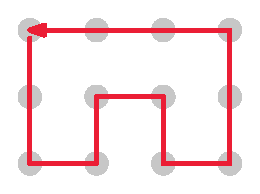
\includegraphics[scale=0.75]{figures/ponder_national_greedytsp_02.eps} \\ 
        ({\hrsp}a{\hrsp})
        
        \vspace{2\baselineskip}
        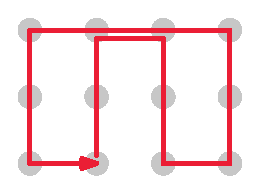
\includegraphics[scale=0.75]{figures/ponder_national_greedytsp_03.eps} \\ 
        ({\hrsp}b{\hrsp})
        
        \vspace{2\baselineskip}
        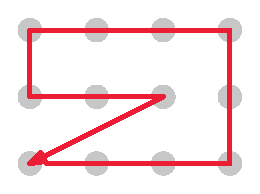
\includegraphics[scale=0.75]{figures/ponder_national_greedytsp_04.eps} \\ 
        ({\hrsp}c{\hrsp})
    \end{center}
}
\begin{center}
    \medskip
    
\includegraphics[]{figures/ponder_national_greedytsp_01.eps}
\end{center}

\noindent
\textbf{\uline{เคสตัวอย่าง}} ให้พิจารณากราฟข้างต้น ซึ่งประกอบด้วยจุดบน Euclidean space 
ที่เรียงเป็นตารางสี่เหลี่ยมผืนผ้า 3 แถว แถวละ 4 จุด\; นอกจากนั้นแต่ละแถวและแต่ละคอลัมน์ห่างกัน 1 หน่วย

\begin{itemize}
\item หากเราโชคดีหน่อย Greedy algorithm อาจจะค้นพบเส้นทาง ({\hrsp}a{\hrsp}) 
    ที่แสดงทางด้าน\ifpageodd{ขวา}{ซ้าย}มือ 
    เส้นทางดังกล่าวมีระยะทางเท่ากับ $\mathrm{12}$ หน่วย ซึ่งเป็น optimal solution
\item แต่หากโชคไม่ค่อยดี Greedy algorithm มีโอกาสพบเส้นทางอื่นเช่น ({\hrsp}b{\hrsp}) หรือ ({\hrsp}c{\hrsp}) 
    ซึ่งมีระยะทางรวมเท่ากับ $\mathrm{14}$ หน่วย 
    และ $\mathrm{11} + \sqrt{\mathrm{5}}\approx\mathrm{13.236}$ หน่วยตามลำดับ
\end{itemize}

\noindent
จงหาเส้นทางที่ Greedy algorithm นี้มีโอกาสค้นพบ ที่มีระยะทางมากกว่า $\dfrac{\mathrm{160}}{\mathrm{9}}$ หน่วย

